\documentclass{article}

% Language setting
% Replace `english' with e.g. `spanish' to change the document language
\usepackage[english]{babel}

% Set page size and margins
% Replace `letterpaper' with `a4paper' for UK/EU standard size
\usepackage[letterpaper,top=2cm,bottom=2cm,left=3cm,right=3cm,marginparwidth=1.75cm]{geometry}

% Useful packages
\usepackage{amsmath}
\usepackage{graphicx}
\usepackage[colorlinks=true, allcolors=blue]{hyperref}

\usepackage{listings}
\usepackage{xcolor}

\lstset{
    basicstyle=\ttfamily\small,
    backgroundcolor=\color{gray!10},
    frame=single,
    breaklines=true
}

\title{Projeto 2 de Segurança e Confiabilidade - Parte 1: Iptables}
\author{João Rodrigues 61789 \\ Rafael Figueiredo 61813 \\Guilherme Sarreira 61860}

\begin{document}
\maketitle

\section{Introdução}

No âmbito deste projeto, pretende-se configurar a firewall da máquina \textit{SperServ} utilizando o comando \texttt{iptables}, de forma a garantir um ambiente seguro para a execução do servidor \textit{SpertaServer}, desenvolvido anteriormente no Projeto 1.

A segurança de sistemas passa, em grande parte, pela redução da superfície de ataque, limitando os serviços disponíveis apenas aos estritamente necessários e controlando rigorosamente as comunicações permitidas. Assim, a firewall deverá implementar uma política de filtragem capaz de restringir o tráfego de rede de acordo com os requisitos definidos, permitindo apenas os serviços essenciais ao funcionamento do sistema.

Neste relatório serão apresentadas as regras \texttt{iptables} desenvolvidas para concretizar a política de segurança proposta, bem como a justificação da \textit{default policy} adotada. Serão ainda descritos os métodos de teste utilizados para validar o correto funcionamento das regras implementadas, acompanhados de exemplos e imagens demonstrativas.



\section{Conteúdos}
\subsection{Default Policy Adotada}

Antes da definição das regras específicas da firewall, foi adotada uma \textit{default policy} restritiva, baseada no princípio de \textit{deny by default}. Assim, todo o tráfego que não corresponda explicitamente a uma regra permitida será automaticamente bloqueado.

As políticas por omissão configuradas foram as seguintes:

\begin{itemize}
    \item \texttt{INPUT: DROP}
    \item \texttt{OUTPUT: DROP}
\end{itemize}

Esta abordagem foi escolhida por se adequar melhor aos objetivos do projeto, uma vez que a principal preocupação consiste em garantir que apenas o tráfego estritamente necessário seja permitido. Ao bloquear, por omissão, todas as comunicações não explicitamente autorizadas, reduz-se significativamente a superfície de ataque da máquina \textit{SperServ}, aumentando assim o nível de segurança do sistema.

Desta forma, apenas os serviços e comunicações definidos nos requisitos do projeto foram posteriormente autorizados através de regras específicas do \texttt{iptables}.

\subsection{Regras Iptables Implementadas}

Nesta secção apresentam-se as regras \texttt{iptables} utilizadas para implementar a política de segurança especificada no enunciado do projeto.
sudo iptables -A OUTPUT -m state --state ESTABLISHED,RELATED -j ACCEPT
\subsubsection{Permitir pings provenientes das máquinas SperAdm e CondAdm}

\begin{lstlisting}
sudo iptables -A INPUT -s 10.0.0.3 -p icmp -j ACCEPT
sudo iptables -A INPUT -s 10.0.3.2 -p icmp -j ACCEPT
\end{lstlisting}
sudo iptables -A OUTPUT -p icmp --icmp-type echo-reply -d 10.0.3.2/24 -j ACCEPT
Estas regras permitem que a máquina \textit{SperServ} responda a pedidos de \textit{ping} provenientes das máquinas \textit{SperAdm} e \textit{CondAdm}.

\subsubsection{Permitir pings provenientes da sub-rede dos clientes}

\begin{lstlisting}
sudo iptables -A INPUT -s 10.0.1.0/24 -p icmp -j ACCEPT
\end{lstlisting}
sudo iptables -A OUTPUT -p icmp --icmp-type echo-reply -d 10.0.1.0/24 -j ACCEPT
Esta regra permite pedidos ICMP provenientes da sub-rede onde se encontram os clientes \textit{SperCli1} e \textit{SperCli2}.

\subsubsection{Permitir ligações ao servidor SpertaServer pela sub-rede dos clientes}

\begin{lstlisting}
sudo iptables -A INPUT -p tcp -s 10.0.1.0/24 --dport 22345 -j ACCEPT
\end{lstlisting}

A regra acima permite ligações TCP destinadas ao porto 80 apenas a partir da sub-rede dos clientes, possibilitando o acesso ao serviço \textit{SpertaServer}.

\subsubsection{Permitir ligações SSH já estabelecidas}

\begin{lstlisting}
sudo iptables -A INPUT -m state --state ESTABLISHED,RELATED -j ACCEPT
\end{lstlisting}

Esta regra permite a continuação de ligações SSH já estabelecidas, bem como tráfego relacionado.

\subsubsection{Permitir ligações SSH provenientes da máquina Broker}

\begin{lstlisting}
sudo iptables -A INPUT -p tcp -s 10.0.2.4 --dport 22 -j ACCEPT
\end{lstlisting}

A seguinte regra permite ligações SSH à máquina \textit{SperServ} provenientes da máquina \textit{Broker}.


\subsubsection{Permitir ligações SSH provenientes da sub-rede local}

\begin{lstlisting}
sudo iptables -A INPUT -p tcp -s 10.0.0.0/24 --dport 22 -j ACCEPT
\end{lstlisting}

Esta regra permite ligações SSH provenientes da sub-rede local da máquina \textit{SperServ}.

\subsubsection{Permitir comunicações internas (\textit{loopback})}

\begin{lstlisting}
sudo iptables -A OUTPUT -o lo -j ACCEPT
\end{lstlisting}

Esta regra permite tráfego interno na interface \textit{loopback}, garantindo o correto funcionamento de serviços locais do sistema.

\subsubsection{Permitir envio de pings com limite de 4 por segundo}

\begin{lstlisting}
sudo iptables -A OUTPUT -p icmp -d 10.0.0.0/24 \
-m limit --limit 4/second -j ACCEPT

sudo iptables -A OUTPUT -p icmp -d 10.0.0.0/24 -j DROP

sudo iptables -A OUTPUT -p icmp -d 10.0.2.4 \
-m limit --limit 4/second -j ACCEPT

sudo iptables -A OUTPUT -p icmp -d 10.0.2.4 -j DROP
\end{lstlisting}

Estas regras permitem o envio de pedidos ICMP apenas para máquinas da sub-rede local e para a máquina \textit{Broker}, limitando a frequência a um máximo de 4 pings por segundo. Todos os restantes pings são imediatamente descartados.


\subsubsection{Permitir conexão SSH à máquina CondServ}

\begin{lstlisting}
sudo iptables -A OUTPUT -p tcp -d 10.0.3.3 --dport 22 -j ACCEPT
\end{lstlisting}

Esta regra permite que a máquina \textit{SperServ} estabeleça ligações SSH para a máquina \textit{CondServ}.


\subsubsection{Permitir tráfego de ligações já estabelecidas}

\begin{lstlisting}
sudo iptables -A INPUT -m state --state ESTABLISHED,RELATED -j ACCEPT
\end{lstlisting}

Esta regra foi adicionada para garantir o correto funcionamento de ligações já estabelecidas, permitindo o tráfego de resposta associado a conexões previamente autorizadas.

Dado que foi definida uma \textit{default policy} restritiva do tipo \texttt{DROP}, sem esta regra qualquer pacote de retorno pertencente a uma ligação válida (por exemplo, sessões SSH ou comunicações TCP já estabelecidas) seria bloqueado.

Desta forma, a regra \texttt{ESTABLISHED,RELATED} assegura que apenas novas ligações necessitam de ser explicitamente autorizadas, enquanto o tráfego associado a ligações já permitidas é automaticamente aceite, evitando interrupções de comunicação legítima.


\subsection{Métodos de Teste}

Para validar o correto funcionamento das regras implementadas na firewall, foram realizados diferentes testes, de acordo com o tipo de serviço e comunicação em causa.

\subsubsection{Testes a pings dirigidos à máquina SperServ}

Para verificar se a máquina \textit{SperServ} respondia corretamente a pedidos ICMP provenientes de outras máquinas, foi utilizado o comando \texttt{ping} a partir das máquinas de origem. A validação consistiu na observação da receção de respostas (\textit{echo replies}), confirmando assim se a regra de permissão estava corretamente aplicada ou bloqueada quando não autorizada.

\subsubsection{Testes da aplicação SpertaClient/SpertaServer}

A comunicação entre o \textit{SpertaClient} e o \textit{SpertaServer} foi testada recorrendo à aplicação desenvolvida na primeira fase do projeto. A execução do cliente permitiu confirmar se a ligação ao servidor era estabelecida com sucesso apenas a partir das máquinas e sub-redes autorizadas pela firewall.

\subsubsection{Testes de SSH}

Para testar as regras relacionadas com o serviço SSH, foi iniciado o serviço na máquina \textit{SperServ} ou \textit{CondServ} através do comando:

\begin{lstlisting}
sudo /usr/sbin/sshd -D
\end{lstlisting}

Posteriormente, foi realizado um teste de ligação com:

\begin{lstlisting}
ssh -X 10.0.0.2
\end{lstlisting}

Este teste permitiu validar se as restrições definidas para acessos SSH estavam a ser corretamente aplicadas.

\subsubsection{Testes de comunicação de saída (ping a partir do servidor)}

Para testar as regras de saída da máquina \textit{SperServ}, nomeadamente o envio de \textit{pings} para outras máquinas, foi utilizado o seguinte comando:

\begin{lstlisting}
ping -i 0.1 10.0.0.3
\end{lstlisting}

Este teste permitiu verificar não só a conectividade de saída, mas também a aplicação do limite de taxa definido (máximo de 4 pings por segundo), confirmando o correto funcionamento da regra de limitação de tráfego ICMP.



\subsection{Evidências (Screenshots/Prints)}

\begin{figure}[h]
    \centering
    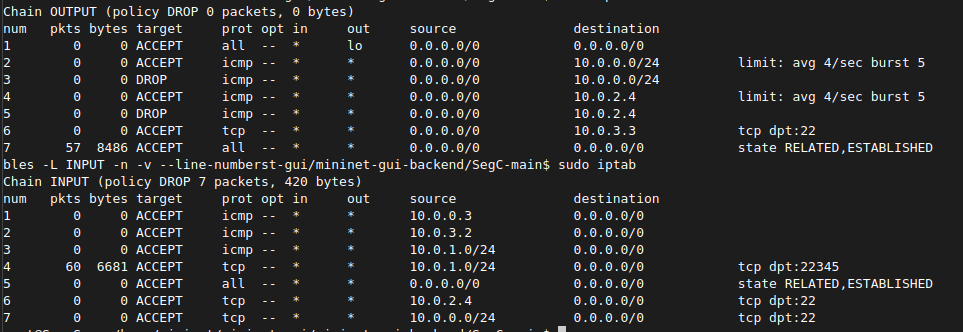
\includegraphics[width=0.8\linewidth]{regras.png}
    \caption{Listagem das regras \texttt{iptables} configuradas na máquina \textit{SperServ}, evidenciando as políticas e permissões implementadas.}
    \label{fig:regras}
\end{figure}

\begin{figure}[h]
    \centering
    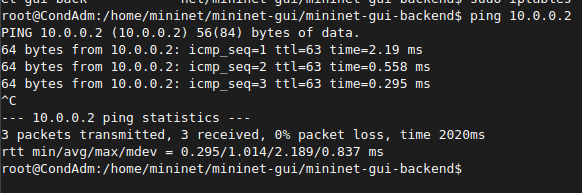
\includegraphics[width=0.8\linewidth]{pings.png}
    \caption{Teste de conectividade ICMP a partir de máquinas autorizadas, demonstrando a correta receção de respostas por parte do \textit{SperServ}.}
    \label{fig:pings}
\end{figure}

\begin{figure}[h]
    \centering
    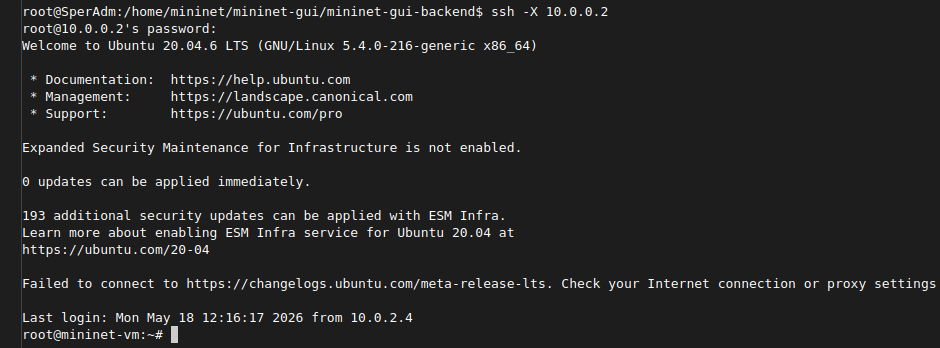
\includegraphics[width=0.8\linewidth]{ssh.png}
    \caption{Teste de ligação SSH à máquina \textit{SperServ}, validando as regras de acesso remoto definidas na firewall.}
    \label{fig:ssh}
\end{figure}

\begin{figure}[h]
    \centering
    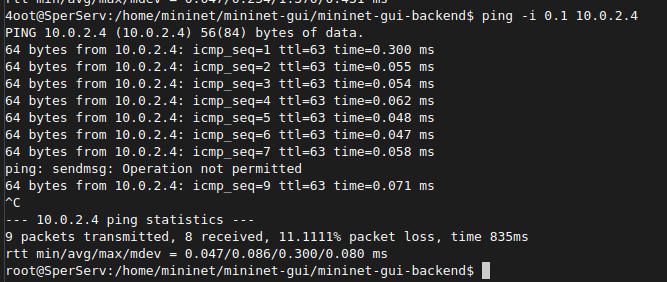
\includegraphics[width=0.8\linewidth]{ping.png}
    \caption{Teste do limite de envio de pacotes ICMP, evidenciando perda de pacotes quando a frequência excede o máximo permitido de 4 pings por segundo.}
    \label{fig:pinglimit}
\end{figure}

\begin{figure}[h]
    \centering
    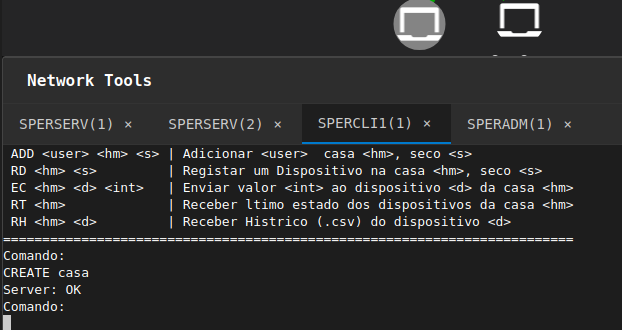
\includegraphics[width=0.8\linewidth]{spertaCliente.png}
    \caption{Execução da aplicação \textit{SpertaClient}, comprovando o estabelecimento de comunicação com o servidor \textit{SpertaServer}.}
    \label{fig:spertaclient}
\end{figure}

\section{Observações e Dificuldades}

Durante a realização do projeto, foram encontradas algumas dificuldades relacionadas com o ambiente de trabalho disponibilizado. Em particular, o terminal do \textit{webshell} do Mininet apresentava problemas de formatação dos comandos introduzidos, dificultando a leitura e interpretação das regras \texttt{iptables}. Esta limitação aumentou a complexidade do processo de configuração e validação da firewall.

Adicionalmente, importa referir que a regra definida para permitir ligações entre o \textit{SpertaClient} e o \textit{SpertaServer} foi configurada especificamente para o porto por omissão utilizado pela aplicação, nomeadamente o porto \texttt{22345}. Assim, ligações efetuadas para portos diferentes não são permitidas pelas regras atualmente implementadas.
\end{document}
sudo iptables -P INPUT DROP
sudo iptables -P OUTPUT DROP

sudo iptables -L OUTPUT -n -v --line-numbers
sudo iptables -L INPUT -n -v --line-numbers

sudo iptables -F
sudo iptables -A INPUT -i lo -j ACCEPT

sudo iptables -P INPUT DROP
sudo iptables -P OUTPUT DROP




sudo iptables -A INPUT -s 10.0.0.3 -p icmp -j ACCEPT
sudo iptables -A INPUT -s 10.0.3.2 -p icmp -j ACCEPT
sudo iptables -A INPUT -s 10.0.1.0/24 -p icmp -j ACCEPT

sudo iptables -A INPUT -p tcp -s 10.0.1.0/24 --dport 22345 -j ACCEPT

sudo iptables -A INPUT -m state --state ESTABLISHED,RELATED -j ACCEPT

sudo iptables -A INPUT -p tcp -s 10.0.2.4 --dport 22 -j ACCEPT
sudo iptables -A INPUT -p tcp -s 10.0.0.0/24 --dport 22 -j ACCEPT

sudo iptables -A OUTPUT -o lo -j ACCEPT

sudo iptables -A OUTPUT -p icmp -d 10.0.0.0/24 -m limit --limit 4/second -j ACCEPT
sudo iptables -A OUTPUT -p icmp -d 10.0.0.0/24 -j DROP

sudo iptables -A OUTPUT -p icmp -d 10.0.2.4 -m limit --limit 4/second -j ACCEPT

sudo iptables -A OUTPUT -p icmp -d 10.0.2.4 -j DROP

sudo iptables -A OUTPUT -p tcp -d 10.0.3.3 --dport 22 -j ACCEPT

sudo iptables -A OUTPUT -m state --state ESTABLISHED,RELATED -j ACCEPT

